\documentclass[a4paper,11pt]{article}
\usepackage{color}
\usepackage{graphicx}
\usepackage{subcaption}
\usepackage{amsmath}
\usepackage{tikz}
\usepackage{listings}
\definecolor{codegreen}{rgb}{0,0.6,0}
\definecolor{codegray}{rgb}{0.5,0.5,0.5}
\definecolor{codepurple}{rgb}{0.58,0,0.82}
\definecolor{backcolour}{rgb}{0.95,0.95,0.92}
 
\lstdefinestyle{mystyle}{
    backgroundcolor=\color{backcolour},   
    commentstyle=\color{codegreen},
    keywordstyle=\color{magenta},
    numberstyle=\tiny\color{codegray},
    stringstyle=\color{codepurple},
    basicstyle=\footnotesize,
    breakatwhitespace=false,         
    breaklines=true,                 
    captionpos=b,                    
    keepspaces=true,                 
    numbers=left,                    
    numbersep=5pt,                  
    showspaces=false,                
    showstringspaces=false,
    showtabs=false,                  
    tabsize=2
}
 
\lstset{style=mystyle}
\usetikzlibrary{automata,positioning}

\graphicspath{ {images/} }
\begin{document}
\title{\color{red}CARNEGIE MELLON UNIVERSITY\\
APPLIED STOCHASTIC PROCESSES  (COURSE 18-751)\\
HOMEWORK 3}
\author{Daniel Marew}
\date{\today}
\clearpage\maketitle

\thispagestyle{empty}
\newpage
I collaborated with :\\
\hspace*{6cm}
Nebyou Yismaw\\
\hspace*{6cm}
Daniel    Nkemelu\\
\hspace*{6cm}
Agatha Niwomugizi
\thispagestyle{empty}
\newpage
\clearpage
\setcounter{page}{1}

\section*{Q.1 \quad Multiplexing}
We can compute the mean 95\% data rate range by approximating it with the normal distribution.
The mean of a bernoulli process   is given by $$\mu=Np$$
where N is the number of trails and p is the probability of success. 
The 95 \% number of users range is given by
\begin{equation}\label{eq:ci}
Np\pm1.96*\sqrt{Np(1-p)}
\end{equation}• 
\subsection*{(a)\quad Base design $N_b = 100$ $R_b = 1Mbps$ and $p_b=0.3$}
$$\mu_b = Np = 100*0.3=30$$
using eqn \ref{eq:ci} number of users range  $$N_bp_b\pm1.96*\sqrt{N_bp_b(1-p_b)}$$ 
from these we get that 95\% of the time the number of users range between 21.01 to 38.98.
The data rate range is just the link data rate divided by the number of users.hence 
The lower limit of the data rate the user will see 95\% of the time $= \frac{1Mbps}{38.98}=25.6kbps\approx26kbps$\\
The upper limit of the data rate the user will see 95\% of the time $= \frac{1Mbps}{21.01}=47.57kbps\approx48kbps$\\\\
Ans. lower limit  = 26kbps upper limit =48kbps , range = 48kbps-26kbps=22kbps
\subsection*{(b)\quad $p_1 \rightarrow 0$ , $\mu_1 = \mu_b$  }
$$\mu_1 =\mu_b= N_1p_1 = 100*0.3=30$$
$$N_1p_1\pm1.96*\sqrt{N_1p_1(1-p_1)} = \mu_1 \pm 1.96 \sqrt{\mu_1} $$ 
since $\mu_1 = N_1p_1$\\ when we substitute all the values we will get \\
from these we get that 95\% of the time the number of users range between 19.264 to 40.73.\\
The upper limit of the data rate the user will see 95\% of the time $= \frac{1Mbps}{19.264}=51.9kbps\approx52kbps$\\
The lower limit of the data rate the user will see 95\% of the time $= \frac{1Mbps}{40.73}=24.55kbps\approx25kbps$\\\\
Ans. lower limit  = 25kbps upper limit =52kbps , range = 52kbps-25kbps=27kbps
\subsection*{(c)\quad $p_1 = p_b=0.3$ , $R_2 = R_bc$ , $N_2 = 100c$, $c=10$ }
$$\mu_1 =\mu_b= N_1p_1 = 100*0.3=30$$
95\% range pf users 
$$N_2p_b\pm1.96*\sqrt{N_2p_b(1-p_b)}=100c*0.3\pm1.96*\sqrt{100c*0.3(1-0.3)} $$ 

$$=30c\pm 1.96*\sqrt{21c} $$ 

when c=10
$$=300\pm 1.96*\sqrt{210} = 300 \pm 28.4 $$ 
from these we get that 95\% of the time the number of users range between 271.59 to 328.40.\\
hence\\\\
The upper limit of the data rate the user will see 95\% of the time $= \frac{1Mbps*10}{271.59}=36.8kbps\approx37kbps$\\
The lower limit of the data rate the user will see 95\% of the time $= \frac{1Mbps*10}{321.40}=31.11kbps\approx31kbps$\\\\
Ans. lower limit  = 31kbps upper limit =37kbps , range = 37kbps-31kbps=6kbps
\subsection*{(d)\quad $p_1 = p_b=0.3$ , $R_2 = R_bc$ , $N_2 = 100c$ ,$c\rightarrow \infty$}
95\% range of datarates\\
$$\frac{R_bc}{100cp_b\pm1.96*\sqrt{100cp_b(1-p_b)}} $$ 
if we divid both numerator and denomerator with c \\
$$\frac{R_b}{100p_b\pm\frac{1.96}{c}*\sqrt{100cp_b(1-p_b)}} $$ 
as $c\rightarrow \infty$ we are left with $$\frac{R_b}{100p_b} $$ 
$$=\frac{1000kbps}{100*0.3}=33.33kpbs$$
The upper and lower limits would be the same 33.33kpbs\\
Ans. upper limit  = lower limit = 33.3kpbs range = 0
\newpage

\subsection*{(e) Compare the designs}
From Table \ref{tab:q1_e} we can clearly observe that the best design is the last one (d).Since our confidence interval is almost zero
we can say with high degree of certainity what the user will be getting 95\% of the time(most of the time).But the problem is, we cannot infinitly add bigger capacity links thus (d) is not a realistic solution.
So I would recommend the design that is the closest to (d) but realstic. In this case, it is New Design 2(c).
\begin{table}
\centering
\hspace*{-3cm}
\begin{tabular}{ |c|c|c|c|} 
\hline
&Lower limit(kbps) & Upper limit(kpbps)\\
\hline
Base Design & 26 & 48\\
\hline
New Design 1& 25 & 52\\
\hline
New Design 2& 31 & 37\\
\hline
New Design 2'& 33.3 &33.3\\
\hline
\end{tabular}
\caption{data rate range for different designs} \label{tab:q1_e}
\end{table}•\\\\
\newpage
\section*{Q.2 Generalized CLT}
\subsection*{(a)\quad Show GCLT reduces to the usual i.i.d version of CLT}
$$Yn = (X_1+X_2+ \dots +X_n-m_n)/Sn$$
where $X_k$ is an independent random variable with $E[X_k]=\mu_k$ and $Var[X_k]= \sigma_k^2$ ,
$m_n = (\mu_1+\mu_2+\dots +\mu_n)/s_n$ and $s_n^2=\sigma_1^2+\sigma_2^2+\dots+\sigma_n^2$\\\\
since i.i.ds have identical distribution the have the same mean and variance\\
i.e $\mu_1=\mu_2=\dots =\mu_n=\mu$ and $\sigma_1^2=\sigma_2^2=\dots=\sigma_n^2=\sigma^2$ \\
$$m_n = (\mu_1+\mu_2+\dots +\mu_n)=n\mu$$
$$s_n^2=(\sigma_1^2+\sigma_2^2+\dots+\sigma_n^2)=n\sigma^2$$
$$Yn = \frac{(X_1+X_2+ \dots +X_n-n\mu)}{\sqrt{n\sigma^2}}$$
$$Yn = \frac{(X_1+X_2+ \dots +X_n-n\mu)}{\sigma\sqrt{n}}$$
hence , GCLT reduces to CLT when \{$X_k$\} are i.i.ds.
\newpage
\subsection*{(b)\quad $X_k$ uniformly distributed from 1 to 5}

\begin{figure}[h]
   \hspace*{-4cm}
    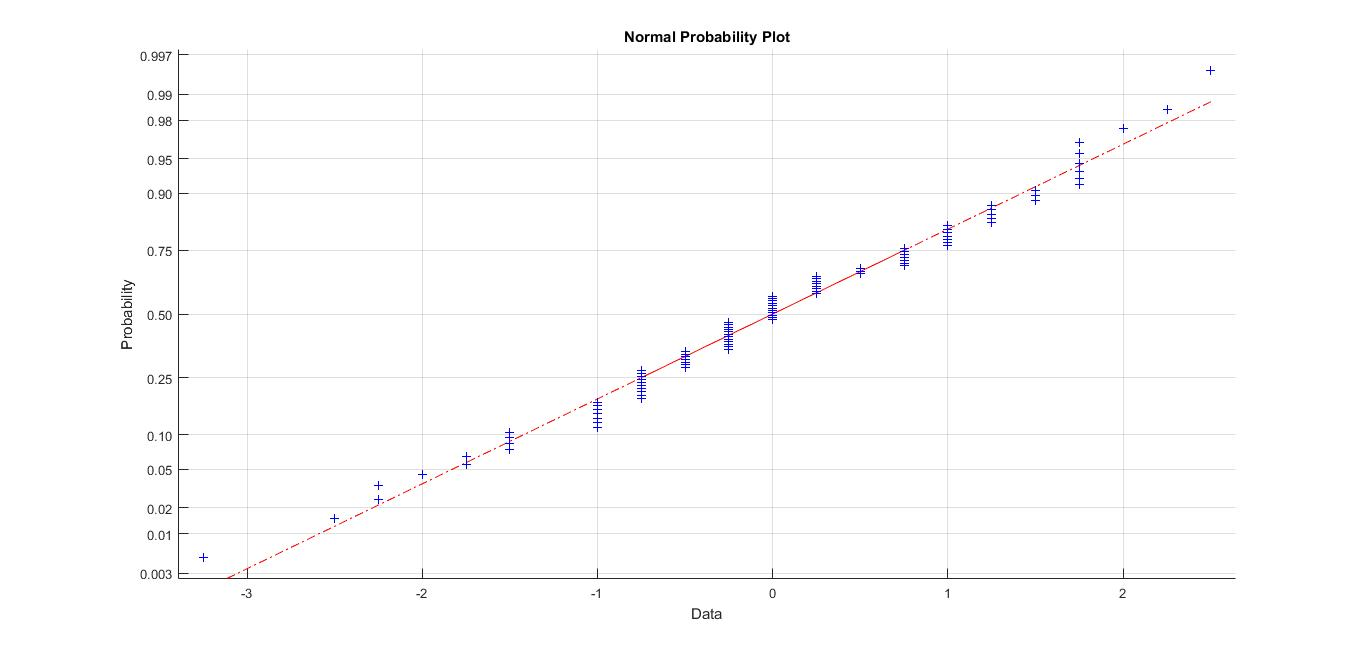
\includegraphics[scale=0.4]{q2_b_1}
    \caption{Normalized histogram Vs pdf of standard normal distribution for (b)}\label{fig:q2_b_1}
\end{figure}
\begin{figure}[h]
   \hspace*{-4cm}
    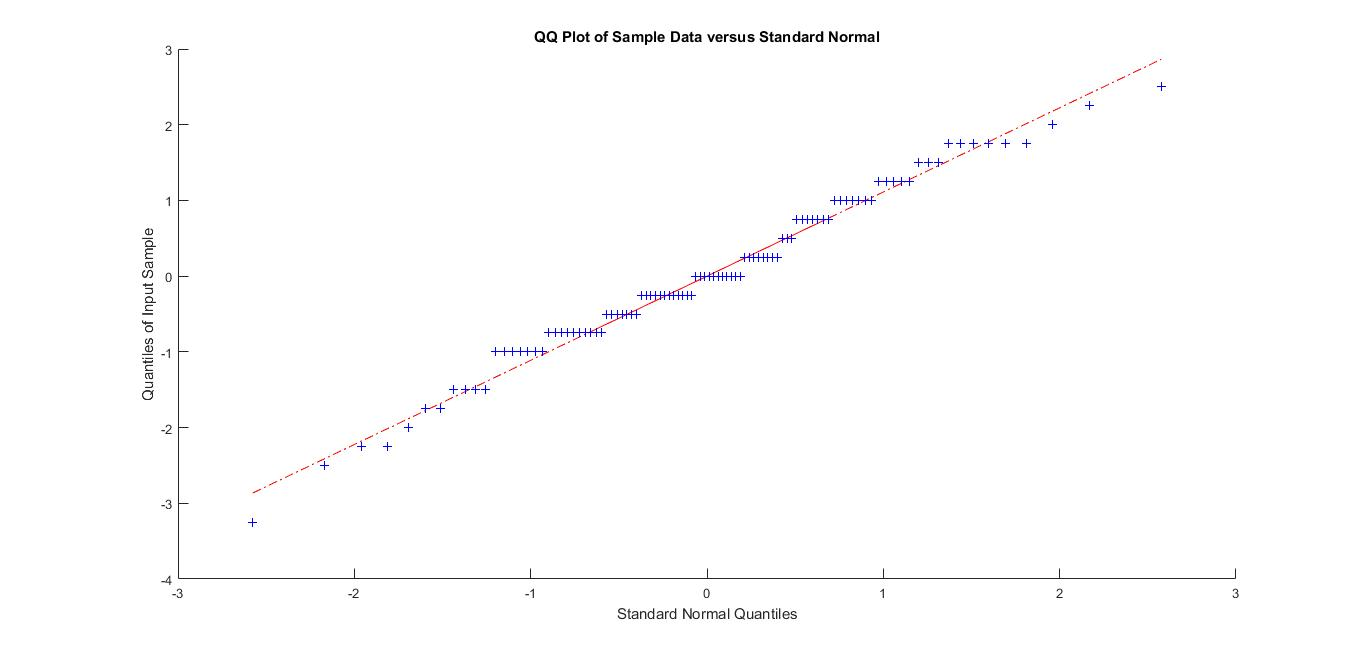
\includegraphics[scale=0.4]{q2_b_2}
    \caption{q-q plot for (b)}\label{fig:q2_b_2}
\end{figure}
\newpage
\clearpage
\subsection*{(c)\quad $X_k$ uniformly distributed from 1 to k}
GCLT applies to (c) if for any $\epsilon >0$ there exists a large enough $n$ such that $\sigma_k<\epsilon S_n$.
$$\sigma_k<\epsilon S_n \implies \sigma_n^2<\epsilon S_n^2$$
the variance for a uniform distribution is given by $$\sigma_k^2 = \frac{(k-1)^2}{12}$$ 
$$S_n^2 = \sigma_1^2 + \sigma_1^2 \dots + \sigma_n^2=\sum_{k=1}^{n}\sigma_k^2=\sum_{k=1}^{n} \frac{(k-1)^2}{12}$$
$$\sum_{k=1}^{n}k^2 = \frac{n(n+1)(n+2)}{6}$$
$$\implies S_n^2 = \frac{(n-1)(n)(n+1)}{72}$$
$\sigma_k<\epsilon S_n$ for any $\epsilon >0$$ \iff $ $\lim_{n \to \infty}\frac{\sigma_k^2}{S_n^2}=0$\\
$max\{\sigma_k\} = \sigma_n$\\
$$\frac{\sigma_n^2}{S_n^2}=\frac{\frac{n-1}{12}}{\frac{(n+1)(n)(n-1)}{72}}=6*\frac{n-1}{n(n+1)}$$
$$=\frac{6*(1-\frac{1}{n})}{(n+1)}$$
hence $$\lim_{n \to \infty }\frac{\sigma_n^2}{S_n^2}=0$$
$\implies$ GCLT applies to (c).

\begin{figure}[h]
   \hspace*{-4cm}
    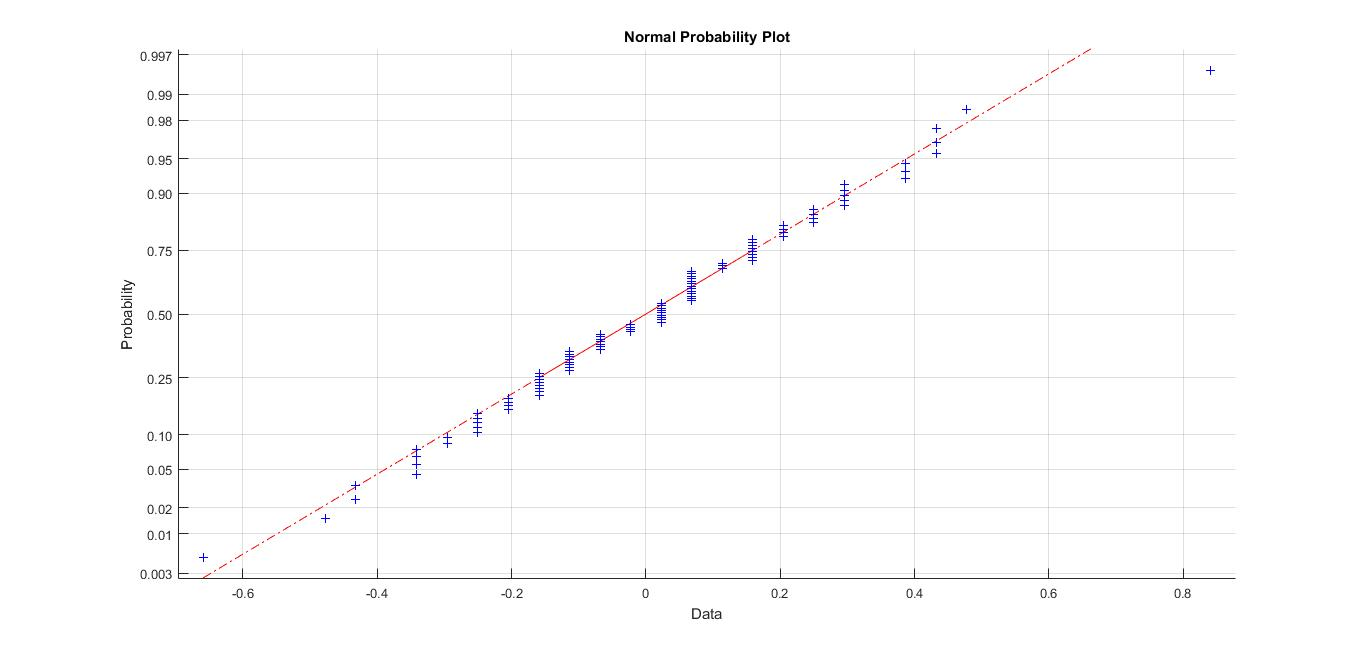
\includegraphics[scale=0.4]{q2_c_1}
    \caption{Normalized histogram Vs pdf of standard normal distribution for (c)}\label{fig:q2_c_1}
\end{figure}
\begin{figure}[h]
   \hspace*{-4cm}
    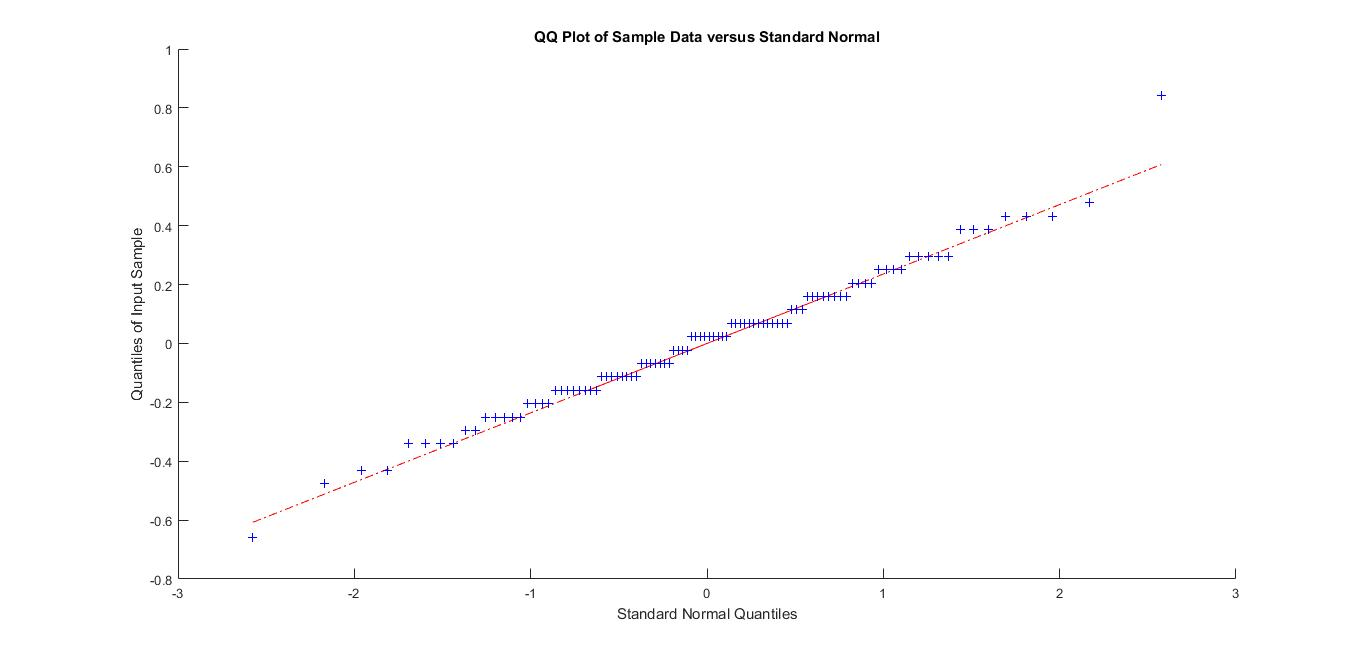
\includegraphics[scale=0.4]{q2_c_2}
    \caption{q-q plot for (c)}\label{fig:q2_c_2}
\end{figure}
\newpage
\clearpage
\subsection*{(d)\quad $X_k=\frac{B_k}{2^k}$  where $B_k$ is a Bernoulli trail with $p=0.5$}
To show that GCLT applies to (d) we need to show for any $\epsilon>0$ there exists a sufficiently large $n$ such that $\sigma_k < \epsilon S_n$.
\[
    B_k= 
\begin{cases}
    1              ,&  p\\
    0 ,             &  1-p
\end{cases}
\]

\[
    X_k= 
\begin{cases}
    \frac{1}{2^k}              ,&  p\\
    0 ,             &  1-p
\end{cases}
\]
$$\mu_k = \frac{1}{2^k}*p + 0*(1-p)  =\frac{p}{2^k} $$
$$\sigma_k^2= E[X_k^2]-E[X_k]^2 = \frac{p(1-p)}{4^k}$$
$$S_n^2 = \sigma_1^2 + \sigma_1^2 \dots + \sigma_n^2=\sum_{k=1}^{n}\sigma_k^2 =\sum_{k=1}^{n}\frac{p(1-p)}{4^k} $$
$S_n^2$ is a geometric series.
as $n \to \infty $ $$S_n^2 = \frac{p(1-p)}{(1-\frac{1}{4})} = p(1-p)*\frac{4}{3}$$
lets take $\epsilon = \frac{1}{4}$ and $k=1$\\
$$\sigma_1^2 = \frac{p}{2}$$
$$\epsilon S_n^2 = \frac{1}{4}*p(1-p)$$
$\frac{p}{2}>\frac{1}{4}*p(1-p) $ for any $p>0 \implies \sigma_1^2 > \epsilon S_n^2 $  when $n \to \infty$\\
Hence we can not find a large enough $n$ such that $\sigma_1<\frac{1}{4}S_n$\\\\
$\implies$ GCLT doesn't apply to (d).
\begin{figure}[h]
   \hspace*{-4cm}
    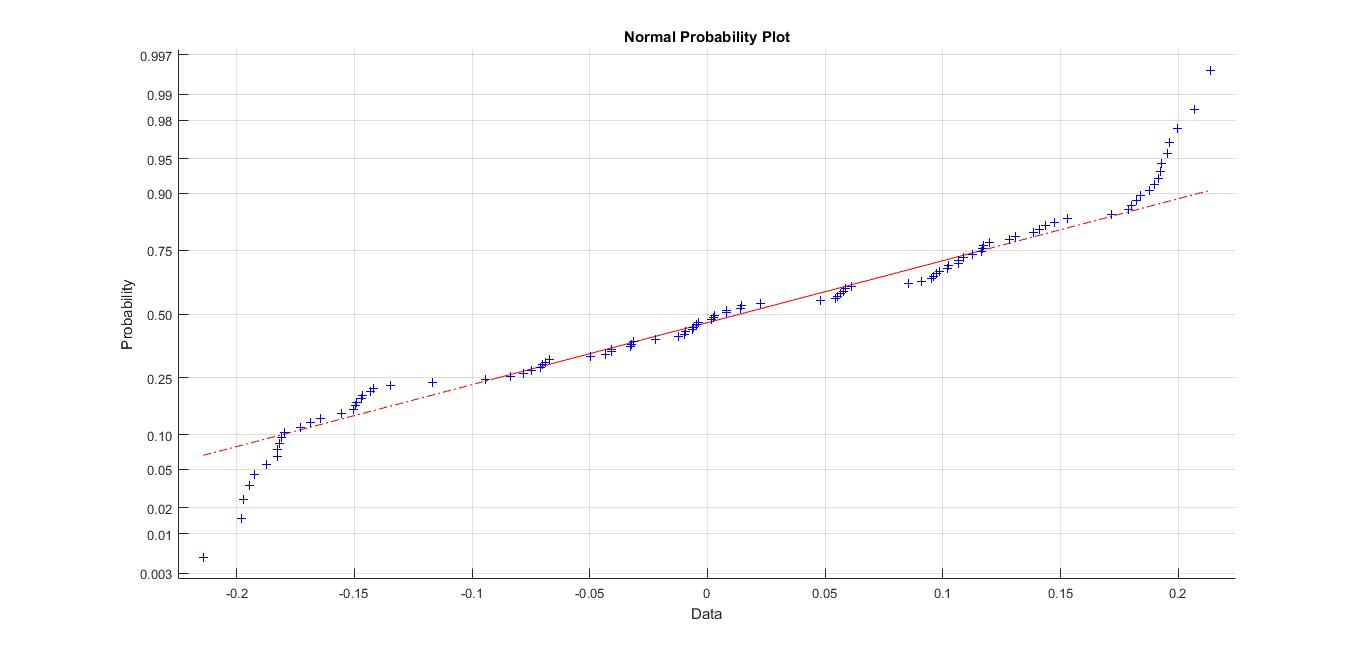
\includegraphics[scale=0.4]{q2_d_1}
    \caption{Normalized histogram Vs pdf of standard normal distribution for (d)}\label{fig:q2_d_1}
\end{figure}
\begin{figure}[h]
   \hspace*{-4cm}
    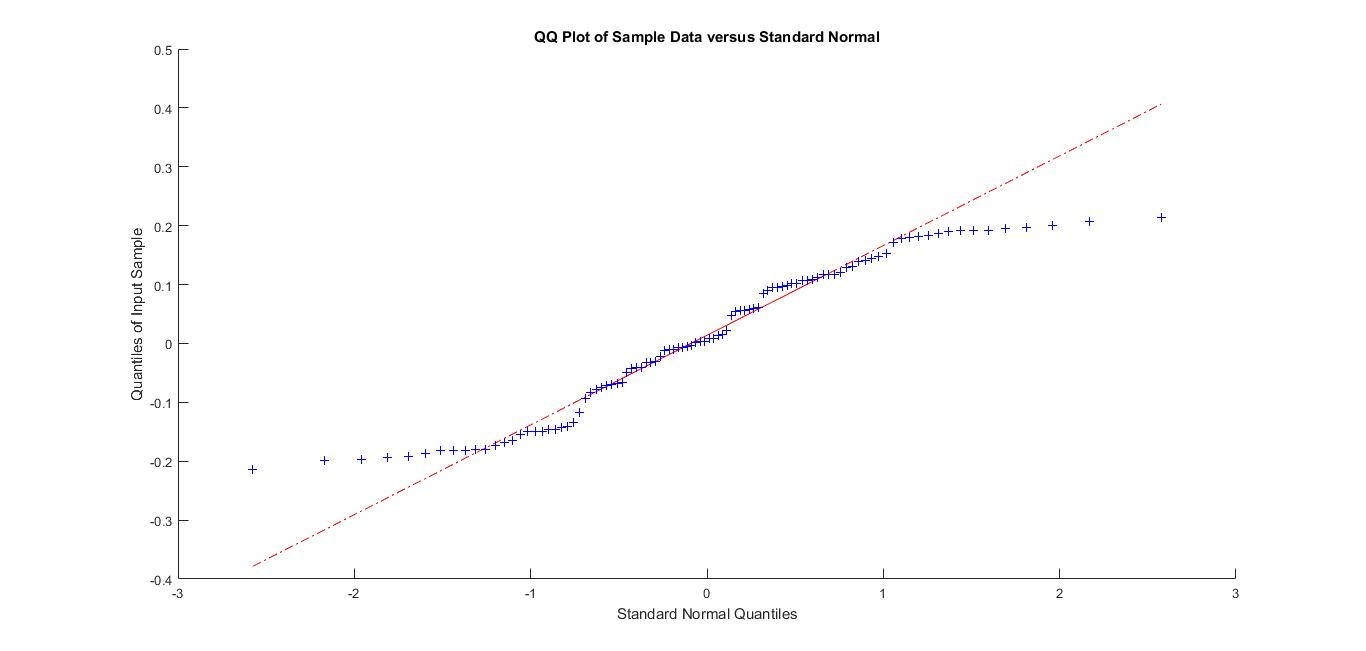
\includegraphics[scale=0.4]{q2_d_2}
    \caption{q-q plot for (d)}\label{fig:q2_d_2}
\end{figure}
\newpage
\clearpage
\subsection*{(e) How well the sum of the first ten elements is approximated by a normal distribution?}
The sum of the first 10 elements in (b) and (c) approximated the normal distribution really well as we can see from the q-q plots (specially (c)) but for (d) the first 10 random variables are not enough to approximate a normal distribution. 
\newpage
\clearpage
\section*{Q3 \quad Buffers}

\subsection*{(a) for $\lambda = 0.1$, $\mu=0.05$, $BufferSize=10$ and $NumberOf Steps=200$ we get Table \ref{tab:q3a} and figure \ref{fig:q3_a} }

\begin{table}
\centering
\begin{tabular}{ |c|c|c|c| } 
\hline
 Average Number of packets in Buffer& 7.81 \\
 \hline
 Fraction of time the buffer is empty& 0.01 \\
 \hline
 The fraction of packet Arrivals that are blocked& 0.00\\
\hline
\end{tabular}
\caption{Question 3b Answer } \label{tab:q3a}
\end{table}•\\\\
\begin{figure}[h]
   \hspace*{-6cm}
    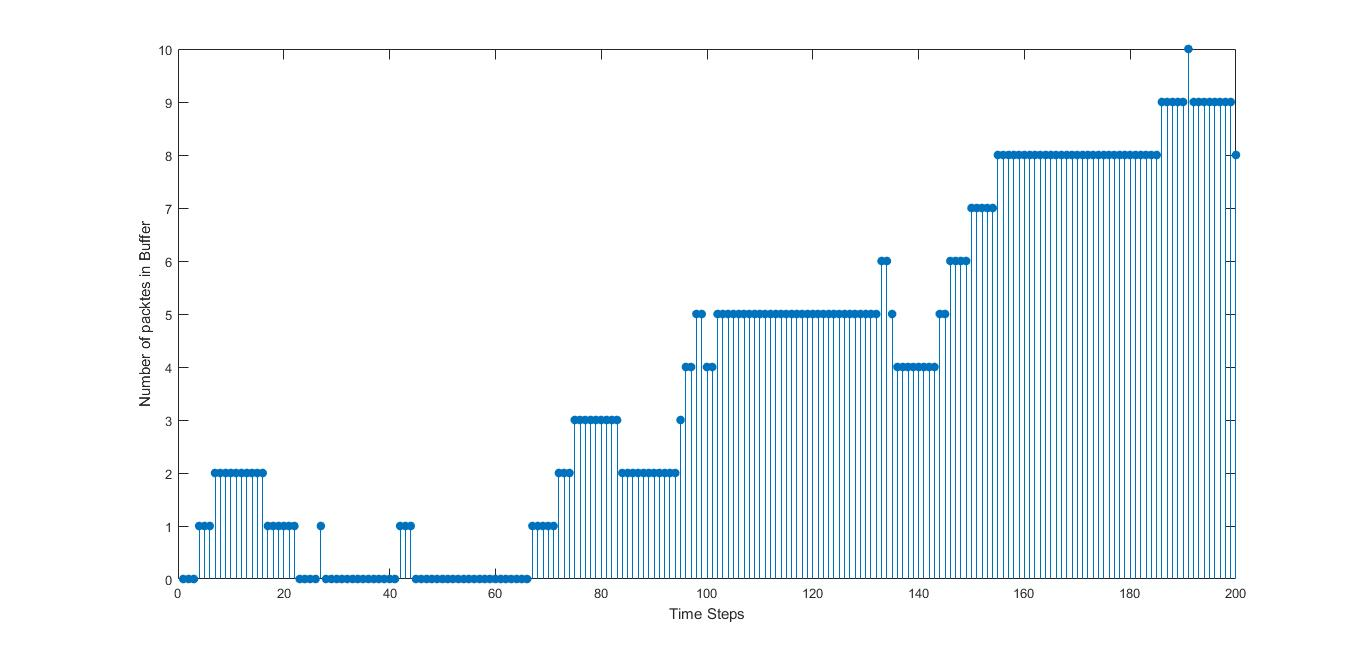
\includegraphics[scale=0.5]{q3_1}
    \caption{Number of packets in the buffer Vs Time steps}\label{fig:q3_a}
\end{figure}
\subsection*{(b) for $\lambda = 0.1$, $\mu=0.01$, $BufferSize=10$ and $NumberOf Steps=200$ we get table\ref{tab:q3b} and figure \ref{fig:q3b} }

\begin{table}
\centering

\begin{tabular}{ |c|c|c|c| } 
\hline
 Average Number of packets in Buffer& 6.23  \\
 \hline
 Fraction of time the buffer is empty& 0.04 \\
 \hline
 The fraction of packet Arrivals that are blocked& 0.2300\\
\hline
\end{tabular}
\caption{Question 3 Answer } \label{tab:q3b}
\end{table}•\\\\
\begin{figure}[h]
   \hspace*{-6cm}
    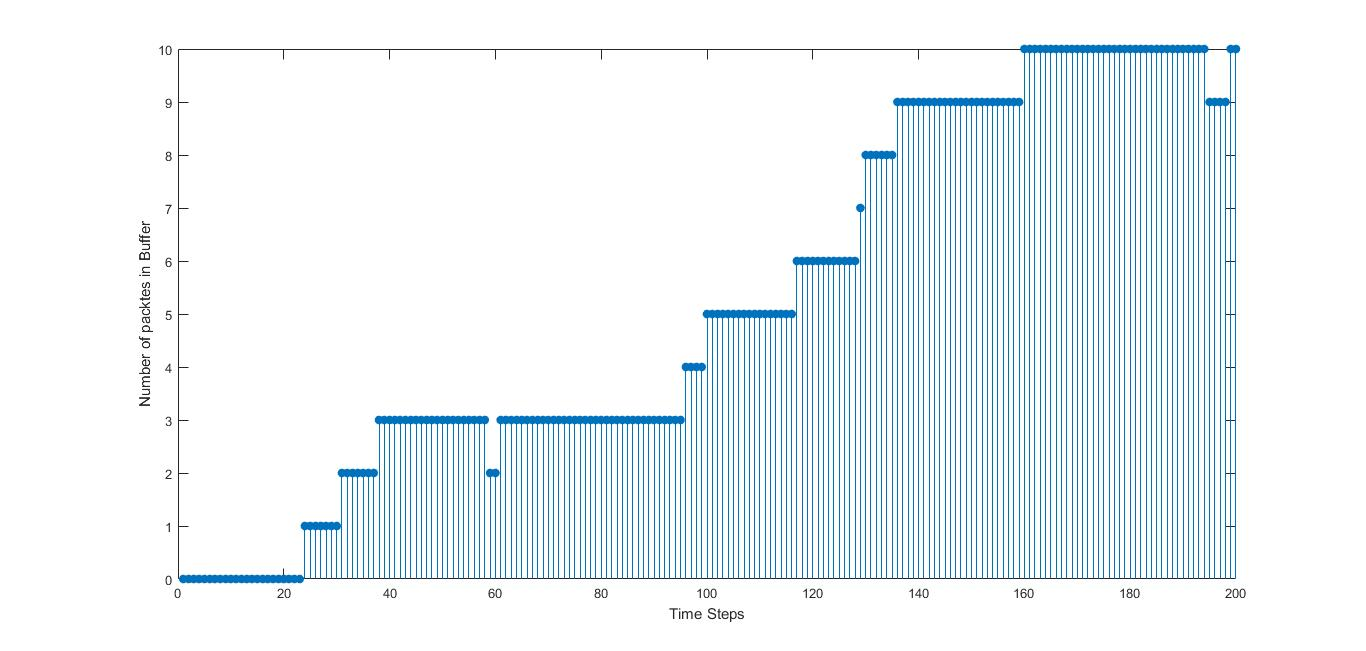
\includegraphics[scale=0.5]{q3_2}
    \caption{Number of packets in the buffer Vs Time steps}\label{fig:q3b}
\end{figure}
\subsection*{(c) Littel Law}
Little Law is given by the following formula \cite{text}\\
\begin{equation}
L = \lambda T
\end{equation}•\\
Where $L$ is the average backlog(the average number of packets in the buffer) , $T$ the delay in the system and $\lambda$ is the average arrival rate.\\\\
hence to get the average delay in the system,
\begin{equation}
T = \frac{L}{\lambda}
\end{equation}•\\
for (a) \\ $$T = \frac{L}{\lambda}=\frac{7.81}{0.1}=78.1$$ timesteps\\
for (b) \\ $$T = \frac{L}{\lambda}=\frac{6.23 }{0.1}=62.3$$ timesteps
\newpage

\begin{appendix}
\section*{Code Appendix}
\subsection*{2. b, c and d}\label{q3code}
\lstinputlisting[language=Octave]{generate_random_variables_d.m}
\lstinputlisting[language=Octave]{generate_random_variables.m}
\lstinputlisting[language=Octave]{computeGCLT.m}
\lstinputlisting[language=Octave]{q2.m}  
\subsection*{3. a and b}\label{q3code}
\lstinputlisting[language=Octave]{get_stochastic_matrix.m}  
\lstinputlisting[language=Octave]{q3.m}  
\lstinputlisting[language=Octave]{simMC.m}  
\lstinputlisting[language=Octave]{discrete.m}  
\end{appendix}•
\begin{thebibliography}{9}


\bibitem{text} 
Jean Walrand. 
\textit{Probability in Electrical Engineering and Computer science}. 
Jean Walrand, 2014.

\end{thebibliography}
\end{document}